\section{Radiography invention: digital radiography}
A quick Google search on ``radiography breakthrough" suffices to show that
digital radiography is the most significant invention for basic radiography in
recent decades. As mentioned earlier in \autoref{ssec:recentradio}, digital
radiographs are much easier to store, copy, post-process share compared to their
analogue siblings. Additionally, unlike radiographic film there is no potential
for over- or underexposure. Instead, the output can be rescaled as needed during
post-processing. Some techniques also allow for a reduced exposure of the
patient, minimizing the risk. The ubiquity of digital scanners these days prove
that the advantages outclass the disadvantages. However, these disadvantages do
exist. Analogue images have a very high inherent resolution, and by examining
them on a lightbox the contrast is unmatched by any kind of computer screen. In
addition, because analogue systems do not use digital electronics, there is no
electronic noise. Digital radiographs do not have necessarily to outclass their
analogue counterparts on these fronts, but they have to achieve a minimum level
to make sure their diagnostic value is not impaired.

\subsection{Defining the technology}
What makes radiography analogue or digital depends on kind of detector used.
Other parts of the scanner such as the X-ray source do not have to be altered
to make the transition. Furthermore, it is not one specific technology that
makes this transition possible. Various components are needed, and for each
of them there are some alternatives as well. On top of that, evolution in other
fields such as digital electronics and computer machinery had to be advanced
enough to take full advantage of the possibilities. 

\begin{figure}[ht]
\begin{center}
  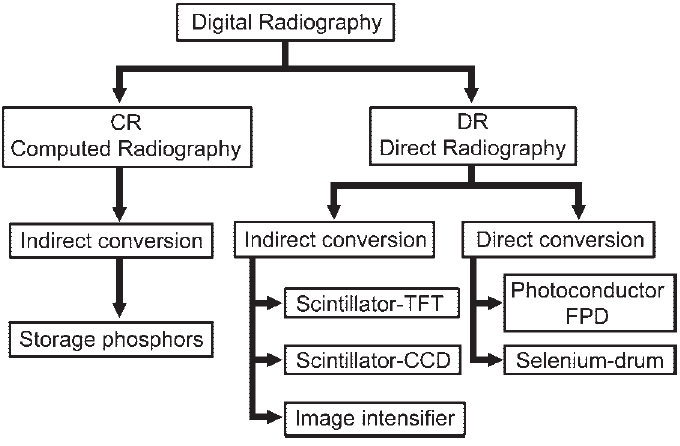
\includegraphics[width=\linewidth]{img/radiohierarchie.png}
  \caption{A systematic overview of various types of digital detectors. CCD =
  chargecoupled device, FPD = flat-panel detector, TFT = thin-film transistor.
  \cite{digitalradio}}
  \label{fig:radiohierarchie}
\end{center}
\end{figure} 

We first discuss the various types in greater detail using
\autoref{fig:radiohierarchie}. The first incarnation of digital radiography -
called computed radiography (CR) - used storage phosphor to temporarily store
the image information, and lasers to read out the values pixel by pixel at a later
stage \cite{digitalradio}. Unfortunately, the physical properties of storage
phosphors severely limited the resolution of the resulting image, reducing their
diagnostic value. The technology underwent many iterations, as shown in
\autoref{tbl:radiotime}.

\begin{table}[ht]
\begin{tabular}{l l}
\hline
Year & Development\\
\hline
1980 & Computed radiography (CR), storage phosphors\\
1987 & Amorphous selenium�based image plates\\
1990 & Charge-coupled device (CCD) slot-scan direct radiography (DR)\\
1994 & Selenium drum DR\\
1995 & Amorphous silicon�cesium iodide (scintillator) flat-panel detector\\
1995 & Selenium-based flat-panel detector\\
1997 & Gadolinium-based (scintillator) flat-panel detector\\
2001 & Gadolinium-based (scintillator) portable flat-panel detector\\
2001 & Dynamic flat-panel detector fluoroscopy�digital subtraction angiography\\
\hline
\end{tabular}
\caption{Timetable of developments in digital radiography \cite{digitalradio}.}
\label{tbl:radiotime}
\end{table}

The alternative to computed radiography is direct radiography (DR). It comes in
two forms, using either direct or indirect conversion. The direct form uses a
photoconductor to convert the incident photons to electrical charges. Typical
semiconductor materials used in photoconductors are amorphous Selenium (a-Se)
and Gadolinium (Gd). In earlier versions the photons were projected onto a
rotating drum and converted to electrical signals using an analog to digital
converter (ADC). Newer versions however use a flat panel detector (FDP) where
the ADC is swapped out for thin-film transistors (TFT, also used in LCD
displays). These TFTs are made of amorphous Silicon (a-Si). Because the used
materials have a very high intrinsic resolution, the final image resolution is
only limited by the kind of detector used.

In indirect conversion DR, an extra element is added between the X-rays and the
actual detector. A common example is a scintillator plate that converts X-rays
into visible light. Alternatively, an image intensifier (II) can be used to
amplify the output. This light can than be captured more easily by a
charge-coupled device (CCD, also used in digital cameras) or a TFT. Because of
the extra step, the point spread function (PSF) increases and the resolution
suffers slightly.

A CCD chip is relatively small so it cannot under normal circumstances record a
whole image at once. Two alternatives are possible. One uses a lens to focus the
rays onto the smaller chip area, but this reduces the image quality. Another
uses a small collimated fan-shaped beam combined with a moving CCD detector.
This system performs comparable to FPDs. One drawback is that this elaborate
setup is not very mobile.

Instead of a CCD, TFTs can also be used in a similar fashion as in direct
conversion DR FPDs. Only this time a scintillator is added. These scintillators
use either Cesium Iodide (CsI) or Gd-based crystals. Contrary to Gd, CsI
crystals can be structured, improving the image quality. The trade-off is their
brittleness, making them less portable.

For the actual assessment, we will focus on both direct and indirect FPDs.

\subsection{Assessing novelty in functionality}
\begin{table}[h]
\centering
\begin{tabular}{l l}
\hline
\multicolumn{2}{|c|}{Novelty in functionality} \\
\hline
A. Novelty of components & B. Novelty in natural effects exploited\\
A1) & B1)\\ 
A2) & B2)\\ 
\hline
\end{tabular}
\caption{Novelty in functionality scores}
\label{tbl:funcscores1}
\end{table}

\subsection{Assessing novelty in origins}
\begin{table}[h]
\centering
\begin{tabular}{l l}
\hline
\multicolumn{2}{|c|}{Novelty in knowledge origins} \\
\hline
A. Novelty of scientific origins & B. Novelty of technological origins\\
A1) & B1)\\ 
A2) & B2)\\ 
\hline
\end{tabular}
\caption{Novelty in knowledge origins scores}
\label{tbl:origscores1}
\end{table}

\subsection{Assessing technological impact}
\begin{table}[h]
\centering
\begin{tabular}{l l l}
\hline
\multicolumn{3}{|c|}{Technological impact} \\
\hline
A. Performance increase & B. Tech. accumulation & Obsoleting previous tech.\\
A) & B1a) & C)\\ 
   & B1b) & \\ 
   & B2a) & \\
   & B2b) & \\
   & B3a) & \\
   & B3b) & \\
\hline
\end{tabular}
\caption{Technological impact scores}
\label{tbl:impactscores1}
\end{table}